\label{section:foundation}
\subsection{Foundation}
Plotting the raw TDE output yields a point cloud with a complex geometry in $d$-dimensional space. This point cloud is characterized by two main properties: directions of maximum variance and their corresponding magnitudes. The directions give the orientation in space where the data varies, and the magnitudes tell how much the data spreads in each direction. The directions where the data varies the most are exactly where the information lies; on the other hand, noise can be found where very little variation is present.
\begin{figure}[H]
\centering
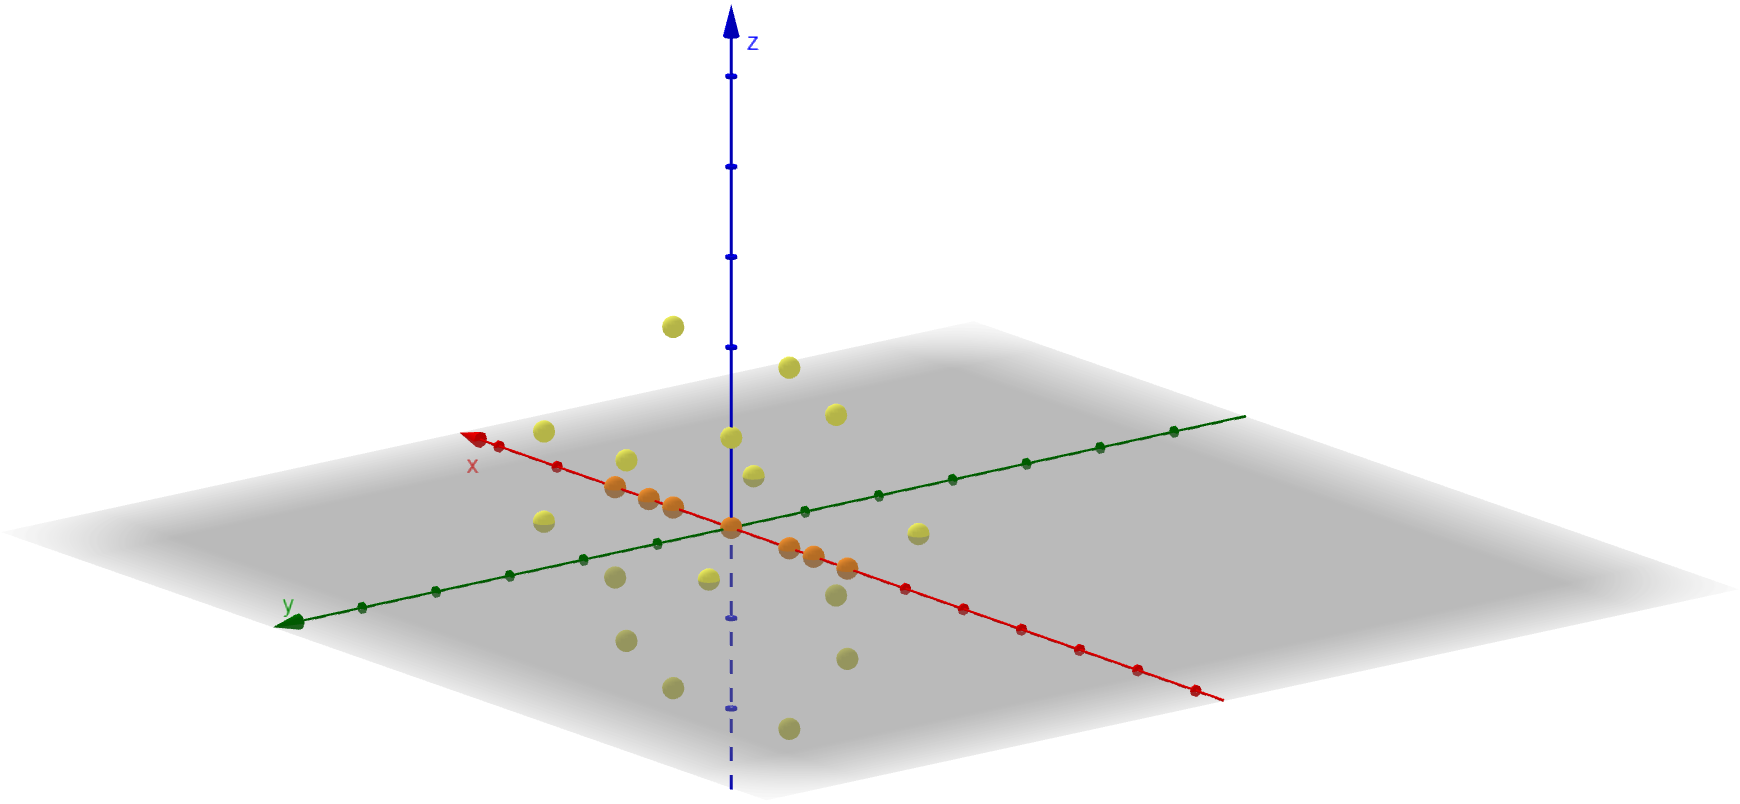
\includegraphics[width=0.7\textwidth]{figures/3dPointcloud.png}
\caption{Visualization of a 3D phase-space point cloud (yellow) and its 1D projection along the principal axis of maximum variance (orange).}
\label{fig:pointCloud}
\end{figure}
One possible approach would be to project all these points onto one single dimension. However, as visualized in Figure~\ref{fig:pointCloud}, when projecting all points onto a single axis, all additional data is lost(demonstrated by the orange points).
When a point $\mathbf{x}$ is projected onto a unit vector $\hat{\mathbf{u}}$, the resulting projected vector $\mathbf{x}'$ lies along $\hat{\mathbf{u}}$ with a magnitude defined by the inner product $\mathbf{x}^T \hat{\mathbf{u}}$:
\begin{equation}
\mathbf{x}' = (\mathbf{x}^T \hat{\mathbf{u}}) \hat{\mathbf{u}}
\end{equation}
The squared inner product $(\mathbf{x}^T \hat{\mathbf{u}})^2$ represents the magnitude of the projection. This squared quantity is minimized when $\mathbf{x}$ is orthogonal to $\hat{\mathbf{u}}$ and maximized when $\mathbf{x}$ is parallel to it. 

The method tries to find the unit vector $\hat{\mathbf{u}}$ that maximizes the sum of these squared projections across the entire dataset. Using the sample covariance matrix
\begin{equation}
\mathbf{C} = \frac{1}{N} \sum_{i=1}^{N} \mathbf{x}_i \mathbf{x}_i^T
\label{eq:covariance_matrix}
\end{equation}
the variance of the projected data is given by $\hat{\mathbf{u}}^T \mathbf{C} \hat{\mathbf{u}}$. Maximizing this variance subject to the constraint $\hat{\mathbf{u}}^T \hat{\mathbf{u}} = 1$ leads to the eigenvalue equation:
\begin{equation}
\mathbf{C}\hat{\mathbf{u}} = \lambda\hat{\mathbf{u}}
\label{eq:eigenvalue_equation}
\end{equation}
This proves that the principal directions of the data correspond to the eigenvectors of the covariance matrix $\mathbf{C}$. Since the variance along any given principal axis equals its corresponding eigenvalue $\lambda$, the eigenvector associated with the largest eigenvalue is the optimal direction that preserves the maximum amount of information.